\documentclass{beamer}

\usetheme{Copenhagen}
\usecolortheme{beaver}
\usefonttheme[onlymath]{serif}

\usepackage[utf8]{inputenc}
\usepackage{graphicx,array,kotex,verbatim,multirow}
\author{김선중}
\date{\today}

%% toc for each section
\AtBeginSection[]
{
 \begin{frame}<beamer>
 \frametitle{}
 \tableofcontents[currentsection,hideallsubsections]
 \end{frame}	
}

%% example environment
\newcounter{chap}
\newcounter{ex}
\makeatletter
\def\th@mystyle{%
    \normalfont % body font
    \setbeamercolor{block title example}{bg=orange,fg=white}
    \setbeamercolor{block body example}{bg=orange!20,fg=black}
    \def\inserttheoremblockenv{exampleblock}
  }
\makeatother
\theoremstyle{mystyle}
\newtheorem*{exam}{\refstepcounter{ex}Example \thechap-\theex}

\newcommand{\pb}[1]%\Phantom + fBox
{\fbox{\phantom{\ensuremath{#1}}}}

\newcommand{\att}{\ensuremath{\text{attn}}}
\newcommand{\sof}{\ensuremath{\text{softmax}}}	

\usepackage{listings,color}
\definecolor{dkgreen}{rgb}{0,0.6,0}
\definecolor{gray}{rgb}{0.5,0.5,0.5}
\definecolor{mauve}{rgb}{0.58,0,0.82}
\lstset{frame=tb,
  language=Python,
  aboveskip=3mm,
  belowskip=3mm,
  showstringspaces=false,
  columns=flexible,
  basicstyle={\small\ttfamily},
  numbers=none,
  numberstyle=\tiny\color{gray},
  keywordstyle=\color{blue},
  commentstyle=\color{dkgreen},
  stringstyle=\color{mauve},
  breaklines=true,
  breakatwhitespace=true,
  tabsize=3
}


\title{Elementary Hyperparameter Tuning}

\setcounter{chap}{2}

\begin{document}
%
\frame{\titlepage}

%
\begin{frame}
\frametitle{Table of Contents}
\begin{enumerate}[1.]
\item
Parameters and Hyperparameters
\begin{itemize}
\item
Parameters
\item
Hyperparameters
\end{itemize}
\item
Four elementary tuning methods
\begin{itemize}
\item
Manual Tuning
\item
Grid Search
\item
Random Search
\item
Bayesian Optimization
\end{itemize}
\item
Survey on papers
\begin{itemize}
\item
Algorithms for Hyper-Parameter Optimization, 2011 (James Bergstra et al., 2011)
\item
Optuna: A Next-generation Hyperparameter Optimization Framework (Takuya Akiba et al., 2019)
\end{itemize}
\end{enumerate}
\end{frame}

%%%
\section{Parameters and Hyperparameters}

%%
\subsection{Parameters}

%
\begin{frame}{Parameters}
Consider a simple neural network, representing  a function \(f:\mathbb R^3\to\mathbb R^3\).
\begin{center}
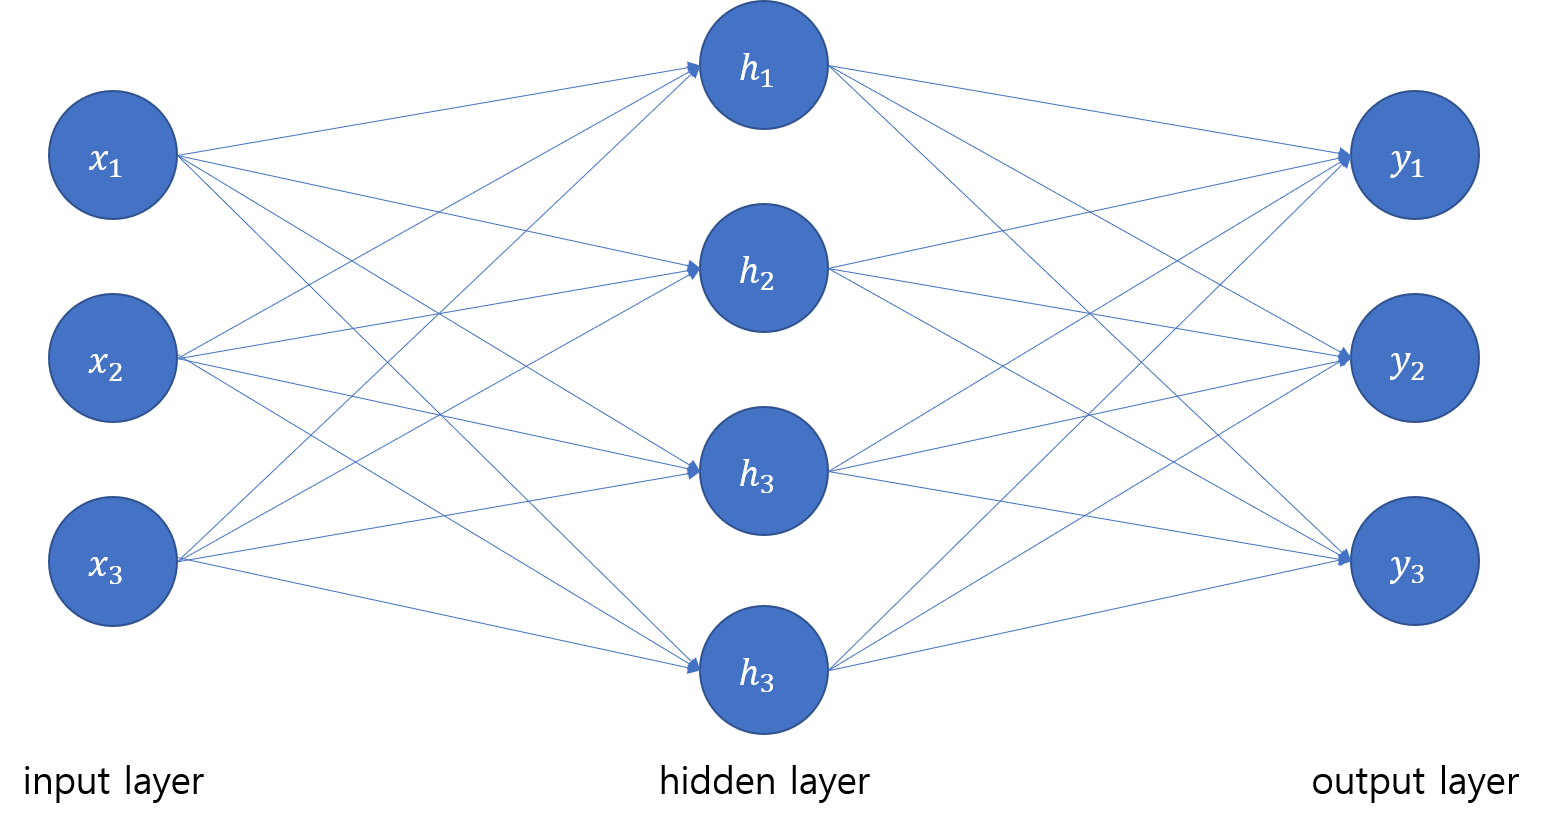
\includegraphics[width=.5\textwidth]{1_1_mlp}
\end{center}
With two matrices \(W\in\mathbb R^{3\times 4}\) and \(W'\in\mathbb R^{4\times 3}\), two vectors \(b\in\mathbb R^4\) and \(b'\in\mathbb R^3\) and the sigmoid function \(\sigma(t)=(1+e^{-t})^{-1}\), we have
\begin{equation}\label{f}
f(x)=\sigma(W'\sigma(Wx+b)+b'),
\end{equation}
where \(\sigma\) is evaluated elementwisely.
\end{frame}

%
\begin{frame}{Parameters}
For a dataset \(D=\{(x^n,y^n):x^n,y^n\in\mathbb R^3,n=1,\cdots,N\}\), the cost can be evaluated as
\begin{equation}\label{cost}
C=\sum_{n=1}^N{||f(x^n)-y^n||_2}^2.
\end{equation}
Denote
\begin{align*}
\Theta
&=(W,b,W',b')\\
&=(w_{11},\cdots,w_{34},b_1,b_2,b_3,b_4,w'_{11},\cdots,w'_{43},b'_1,b'_2,b'_3).
\end{align*}
Since \(f\) depends on \(\Theta\), we may think of \(C:\mathbb R^{31}\to\mathbb R\) as a function of \(\Theta\).
\end{frame}

%
\begin{frame}{Parameters}
\begin{itemize}
\item
Using the gradient descent or the likes, we can find an approximated minimum of \(C(\Theta)\).
\item
The optimal \(f^*\) is then obtained from the the minimum argument \(\Theta^*\).
\item
Components \(w_{ij}\), \(b_k\), \(w'_{ij}\), \(b'_k\) of \(\Theta\) are called the learnable parameters, or simply the \alert{parameters}.
\end{itemize}
\end{frame}

%%
\subsection{Hyperparameters}

%
\begin{frame}{Hyperparameters}
\begin{itemize}
\item
We may change the structure of the network slightly to produce a different function \(f\).
\item
Specifically, we can use different \alert{numbers of nodes in the hidden layer}, say, 5, to enhance the performance.
\item
The number of hidden nodes is an example of \alert{hyperparameter}.
\end{itemize}
\begin{center}
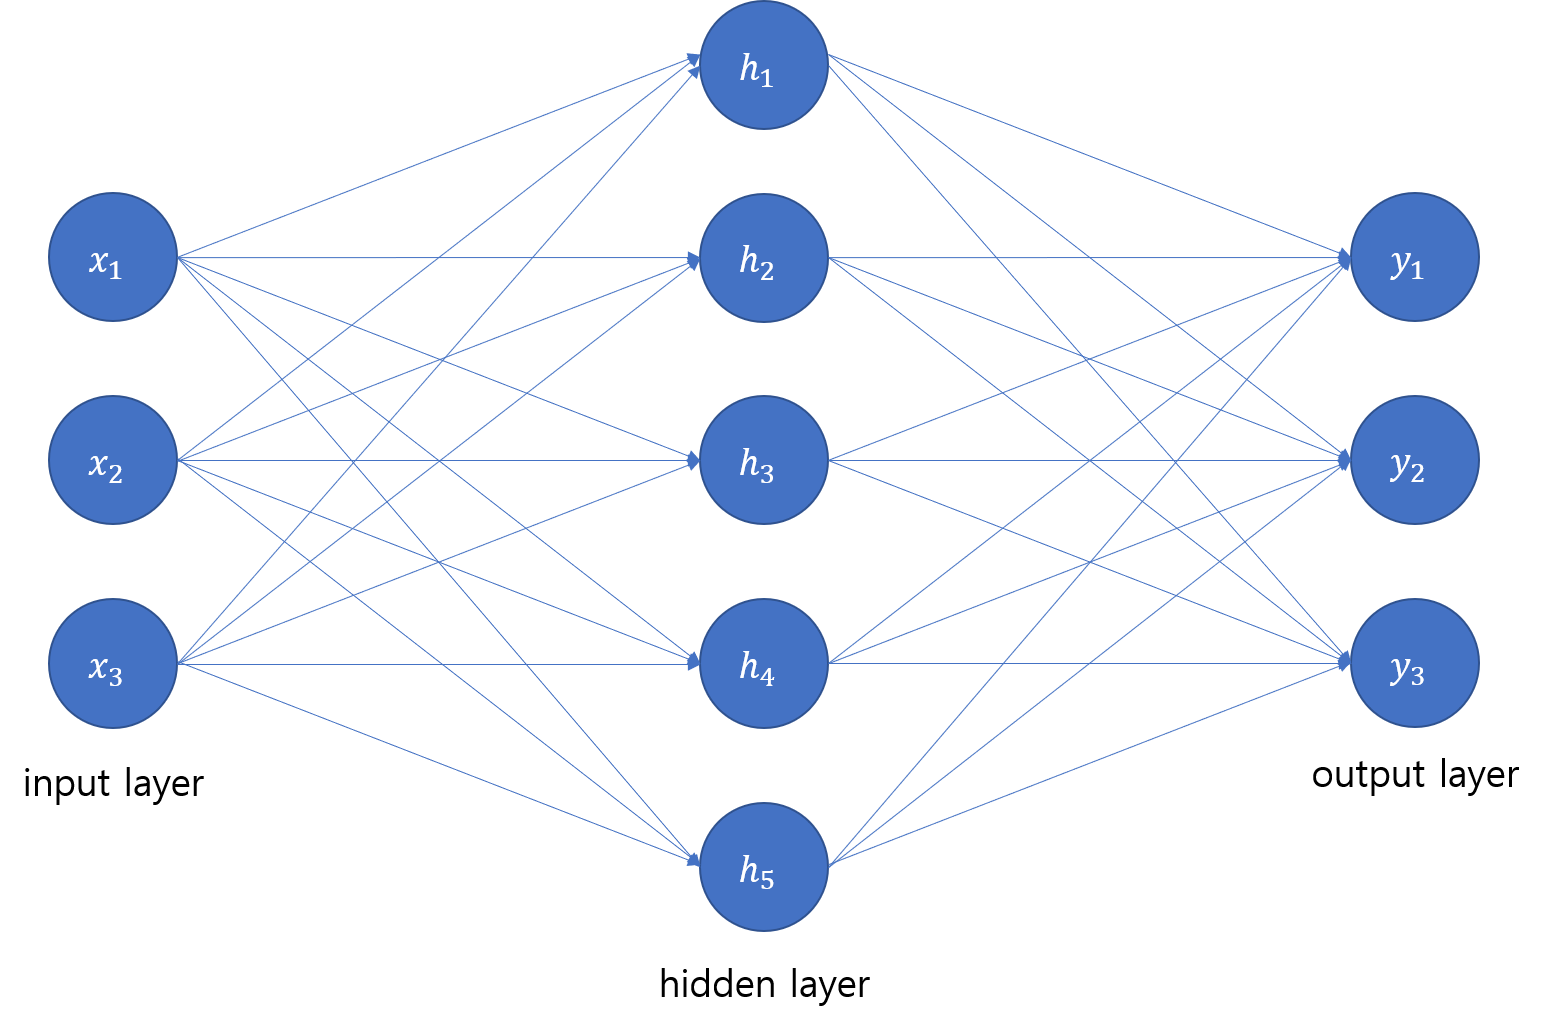
\includegraphics[width=.5\textwidth]{1_2_mlp}
\end{center}
\end{frame}

%
\begin{frame}{Hyperparameters}
\begin{itemize}
\item
Beside the number of hidden nodes, the \alert{learning rate} and the \alert{type of optimizers} is also a hyperparameter.
\item
That is, we may think of an operator \(F\) with its arguements \(\phi_1\)(the learning rate), \(\phi_2\)(the number of hidden nodes) and \(\phi_3\) (the type of optimizer) where
\[F[\phi_1,\phi_2,\phi_3]=f,\]
\end{itemize}
\end{frame}

%
\begin{frame}{Hyperparameters}
\begin{itemize}
\item
Suppose that each hyperparameters \(\phi_i\) has its value in a set ;
\begin{align*}
\phi_1&\in[0.001,0.01]\\
\phi_2&\in\{1,2,3,4,5,6\}\\
\phi_3&\in\{\text{SGD},\text{Adam},\text{RMSprop}\}
\end{align*}
\item
We may think of \(\phi_i\) as random variables.
\item
The sample spaces of \(\phi_i\)'s are
%\(S_i\)'s becomes then the sample spaces.
\begin{align*}
S_1&=[0.001,0.01]\\
S_2&=\{1,2,3,4,5,6\}\\
S_3&=\{\text{SGD},\text{Adam},\text{RMSprop}\}
\end{align*}
\end{itemize}
\end{frame}

%
\begin{frame}{Hyperparameters}
\begin{itemize}
\item
For each \(\Phi=(\phi_1,\phi_2,\phi_3)\), there corresponds a real value \(C(\Theta^*)\).
\item
We are to find the optimal hyperparameters \(\Phi=(\phi_1,\phi_2,\phi_3)\) that minimizes \(C(\Theta^*)\).
\end{itemize}

\bigskip
The task of determining the set of hyperparameter to minimize the cost, given a dataset and the architecture of the model, is called
the \alert{hyperparameter tuning},
hyperparameter optimization, or
hyperparameter selection.
\end{frame}

%
\begin{frame}{Hyperparameters}
%The optimal cost \(C(\Theta^*)\) is then a function of  \(\phi_1\), \(\phi_2\), \(\phi_3)\).
%We are to find the optimal hyperparameters \(\Phi=(\phi_1,\phi_2,\phi_3)\) that minimizes \(C(\Theta^*)\).
Beside
\begin{itemize}
\setlength\itemsep{0pt}
\item
the learning rate
\item
the number of nodes in the hidden layers
\item
the type of optimizer,
\end{itemize}
the followings are also possible hyperparameters ; 
\begin{itemize}
\setlength\itemsep{0pt}
\item
the size of minibatch
\item
the number of epochs
\item
the type of activation function
\item
the type of weight initialization
\item
the dropout parameter
\item
the regularization parameter
\end{itemize}
\end{frame}

%%%
\section{Four elementary tuning methods}

%%
\subsection{Manual Tuning}

%
\begin{frame}{Manual Tuning}
\begin{itemize}
\item
As the most primitive and natural method, we may tune the hyperparameters by hands.
\item
We move from one point in the hyperparameter space to the other, each time evaluating the cost.
\item
There is no general rule for manual tuning.
\end{itemize}
\begin{multline*}
(\phi_1,\phi_2,\phi_3)
\longrightarrow(\phi_1+\epsilon_1,\phi_2,\phi_3)
\longrightarrow({\phi_1}^*,\phi_2,\phi_3)\\
\longrightarrow({\phi_1}^*,\phi_2+\epsilon_2,\phi_3)
\longrightarrow({\phi_1}^*,{\phi_2}^*,\phi_3)
\longrightarrow\cdots
\end{multline*}
\end{frame}

%
\begin{frame}{Manual Tuning}
Advanatges
\begin{itemize}
\item
We can learn the behavior of hyperparameters by heart.
%\item
%We can use your knowledge in another project.
\end{itemize}
Disadvantages
\begin{itemize}
\item
Manual works are required.
\item
There is no general rule.
\end{itemize}
\end{frame}

%%
\subsection{Grid Search}

%
\begin{frame}{Grid Search}
\begin{itemize}
\item
Consider tuning \(\phi_2\) and \(\phi_3\) while \(\phi_1\) is fixed.
\begin{align*}
\phi_2&\in S_2=\{1,2,3,4,5,6\}\\
\phi_3&\in S_3=\{\text{SGD},\text{Adam},\text{RMSprop}\}
\end{align*}
\item
There are \(|S_2|\times|S_3|=6\times 3=18\) possibilities that \((\phi_2,\phi_3)\) can attain.
\begin{center}
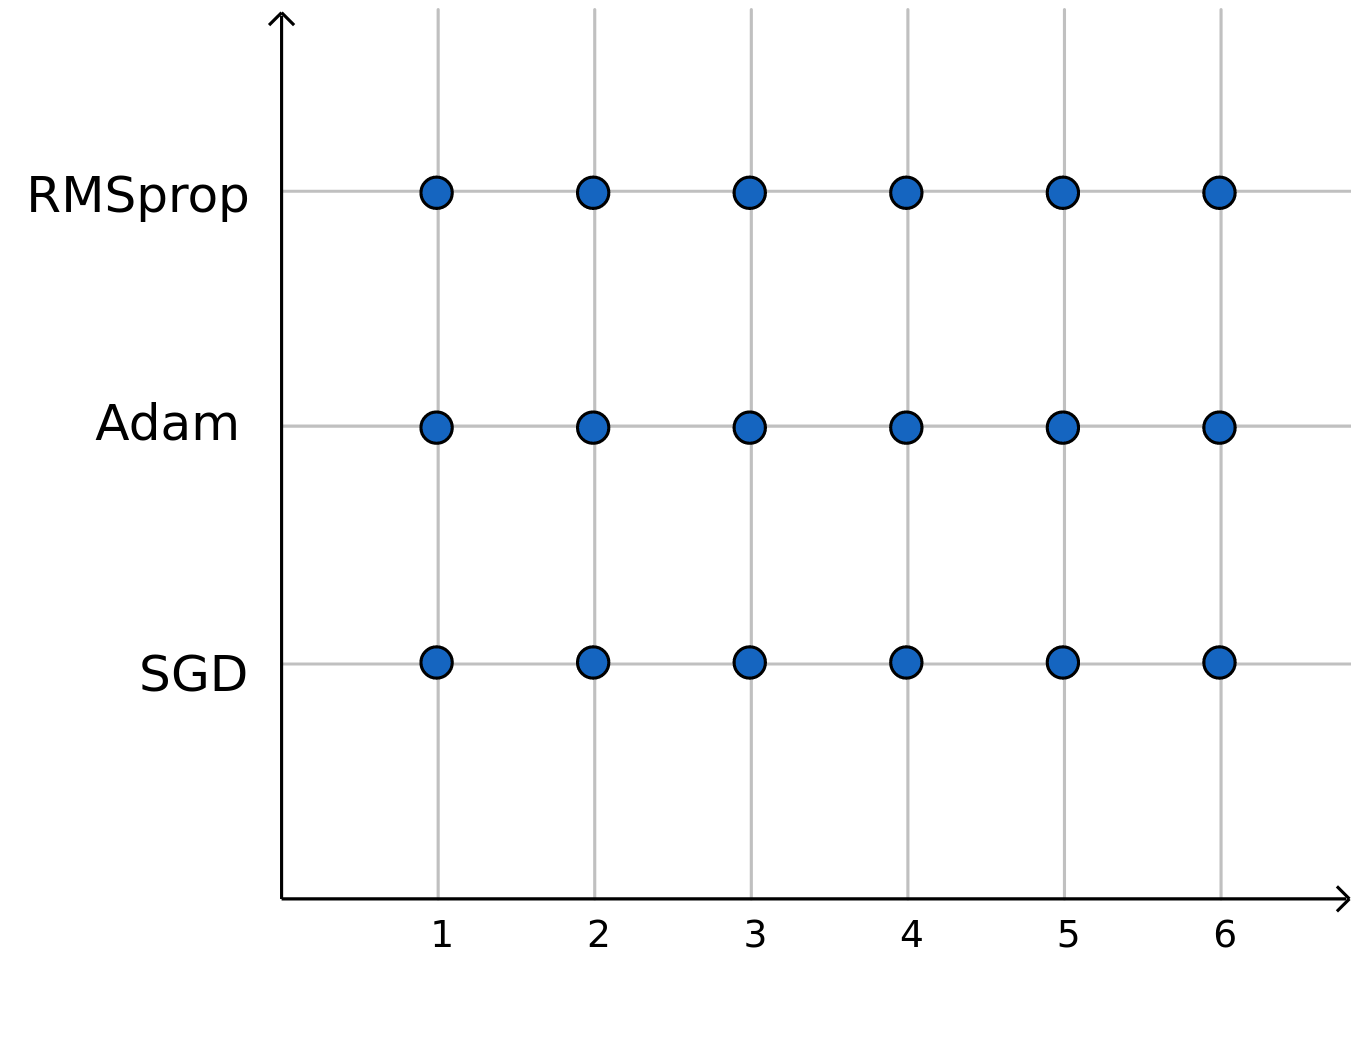
\includegraphics[width=.5\textwidth]{2_1_grid_2d}
\end{center}
%\item
%18 points in the hyperparameter space \(S_1\times S_2\).
\end{itemize}
\end{frame}

%
\begin{frame}{Grid Search}
\begin{itemize}
\item
Consider tuning \(\phi_1\), \(\phi_2\), \(\phi_3\) simultaneously.
\item
Since \(\phi_1\) lies in a (continuous) closed interval \(S_1=[0.001,0.01]\) we need to discretize it ;
\[\phi_1\in\{0.001, 0.005, 0.01\}.\]
\item
There are \(3\times 6\times 3=54\) cases ;\\
i.e. 54 points on the hyperparameter space \(S_1\times S_2\times S_3\).% three dimensional grid.
\item
For each cases, we train the model and test the performance independently.
\item
By comparing all the cost we get, we find the set of optimal hyperparameters and the corresponding cost value.
\end{itemize}
\end{frame}

%
\begin{frame}{Grid Search}
Advanatges
\begin{itemize}
\item
We can cover all possible prospective sets of hyperparameters.
\end{itemize}
Disadvantages
\begin{itemize}
\item
It may take too long ; the running time increase exponentially as the number of types of hyperparameter increases.
\item
There exist holes between grids.
\end{itemize}
\end{frame}

%
\begin{frame}{Grid Search : Code}
\begin{center}
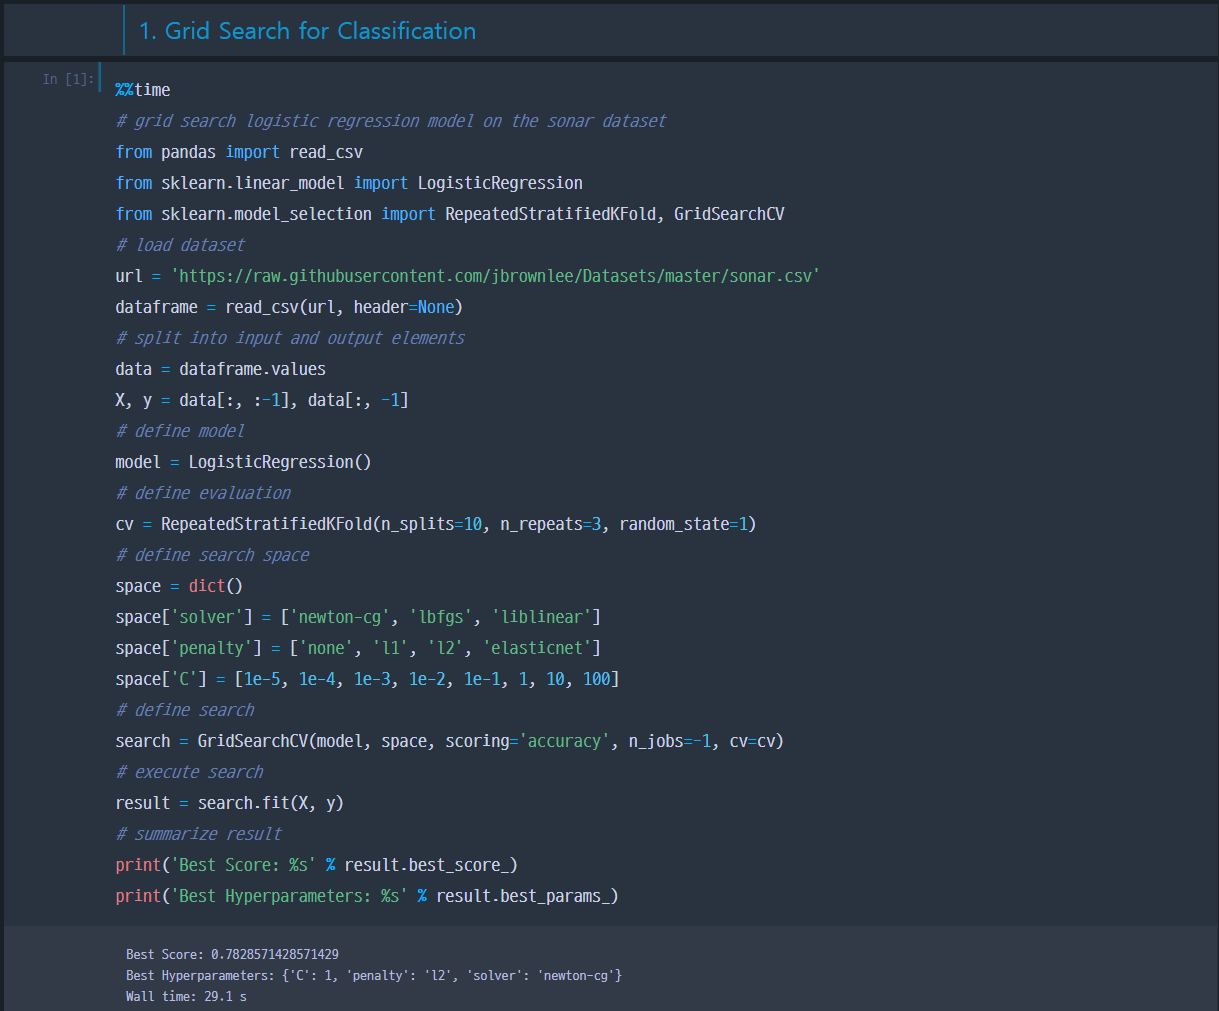
\includegraphics[width=.75\textwidth]{2_2_grid_search}
\end{center}
\end{frame}

%%
\subsection{Random Search}

%
\begin{frame}{Random Search}
\begin{itemize}
\item
Think of the hyperparameters \(\phi_i\) as random variables with adequate distribution.
\item
Sample from the joint distribution of \(\Phi=(\phi_1,\phi_2,\phi_3)\), build a model and test the performance.
\item
We can repeat this procedure multiple times and select the best one as the optimal set of hyperparameters.
\end{itemize}
\end{frame}

%
\begin{frame}{Random Search}
Advanatges
\begin{itemize}
\item
Sampling can find unexpected points in the hyperparameter space with good performance.
\item
To get more accurate model, we simply increase the number of sampling.
\end{itemize}
Disadvantages
\begin{itemize}
\item
If the hyperparameter space is big, then some hyperparameters might not be explored.
\item
We must specify the probability distribution of the sample space in advance.
\end{itemize}
\end{frame}

%
\begin{frame}{Random Search : Code}
\begin{center}
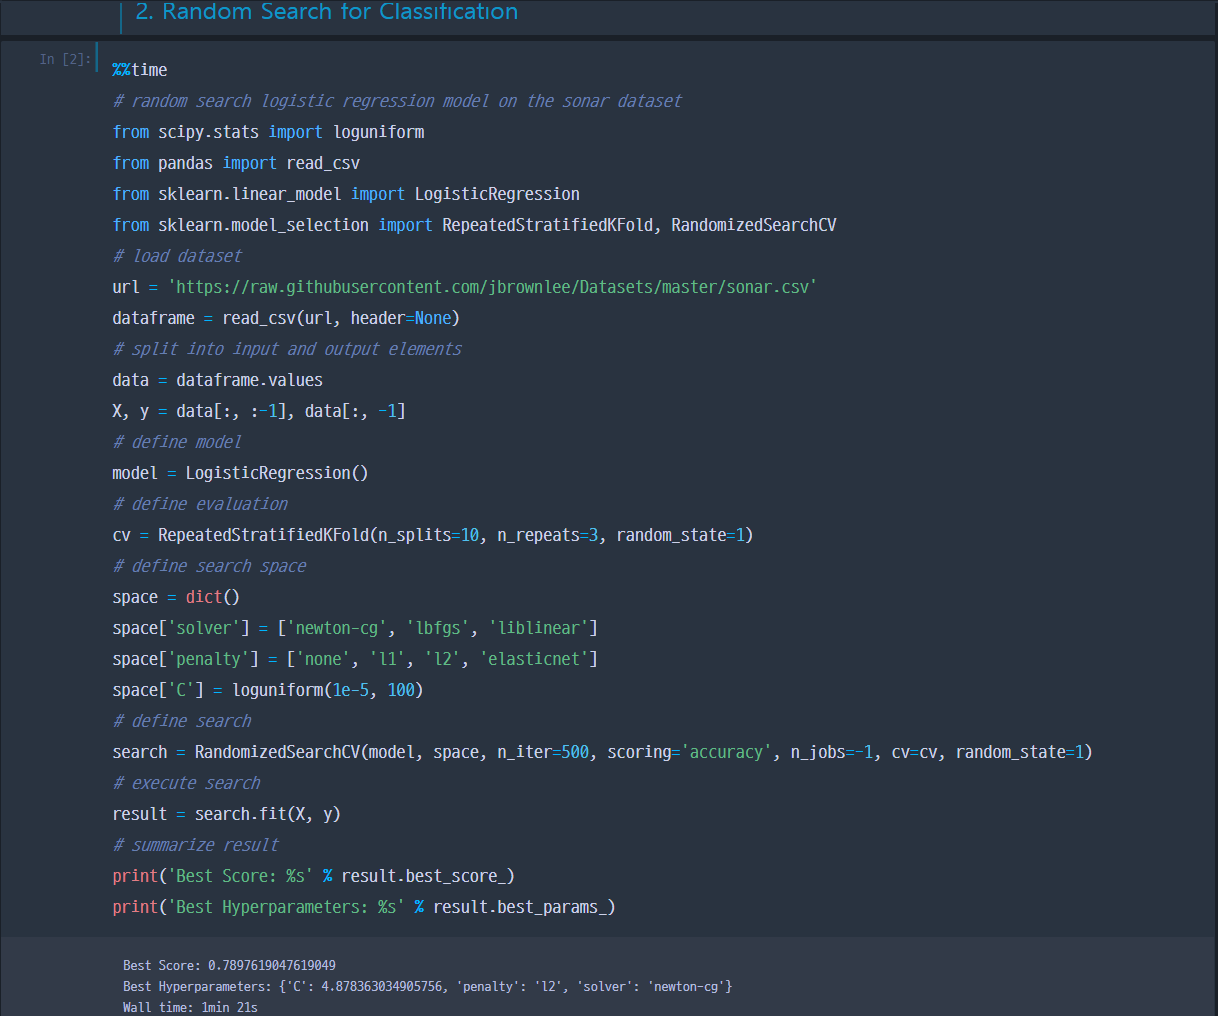
\includegraphics[width=.75\textwidth]{2_3_random_search}
\end{center}
\end{frame}

%
\begin{frame}{Grid Search vs Random Search}
\begin{center}
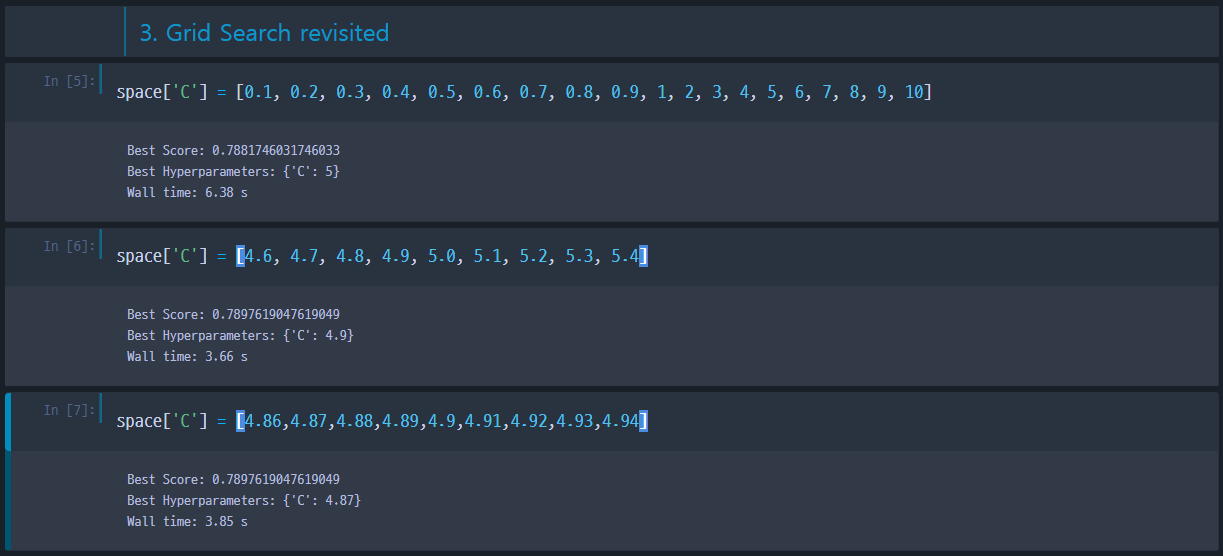
\includegraphics[width=.75\textwidth]{2_4_grid_search_revisit}
\end{center}
\begin{itemize}
\item
Grid method takes less time (29.1s, 6.38s, 3.66s, 3.85s) than random search(1min 21s).
\item
But random search requires just one step to implement and we don't have to set the grid carefully like we did in grid method.
\item
Morever, it produces quite an accurate result, compared to the random search.
\end{itemize}
\end{frame}

%%
\subsection{Bayesian Optimization}

%
\begin{frame}{Bayesian Optimization}
\begin{itemize}
\item
A drawback of random search : \alert{we must specify the probability distribution of the sample space in advance.}
\item
In bayesian optimization, the probability distribution evolves from one to another.
\item
Specifically, given a \alert{prior} distribution \(P(f)\), we get the \alert{posterior} distribution \((f|D)\) iteratively.
\item
Bayes Rule :\\
\[P(f|D)\propto P(D|f)P(f).\]
\item
More detailed explanation and the code will be covered in the final presentaion.
\end{itemize}
\end{frame}

%%
\section{An Overview of Bayesian Optimizaton}
\begin{frame}{An Overview of Bayesian Optimizaiton}
\begin{itemize}
\item
Bayesian optimization is a method for maximizing (or minimizing) a function \(f:A\to\mathbb R\) where \(A\subset\mathbb R^d\).
Sometimes we write
\[\max_{x\in A}f(x).\]
\item
The \alert{objective function} \(f\) is unknown, we are to sample from the domain \(A\) using \alert{surrogate function} and \alert{acquisition function} to achieve our goal.
\end{itemize}
\end{frame}

%
\begin{frame}{An Overview of Bayesian Optimizaiton}
In our problem, we are assuming the followings;
\begin{itemize}
\item
\(d\), the dimension of the domain, is assumed to be less than 20.
\item
\(x\), the independent variable, is assumed to be within a simple domain \(A\) like \(k\)-cube \(\prod_{i=1}^k[a_i,b_i]\).
\item
\(f\) is assumed to be a good function in a sense that it is (Lipschitz) continuous.
But it is not differentiable.
So it is impossible to approximate \(f\) using its derivatives or its second derivatives.
\item
Still, \(f\) is really complicated function, so one can not evaluate the value in low cost.
And it lacks special structure like concavity or linearity.
\end{itemize}
\end{frame}

%
\begin{frame}{Overview of Bayesian Optimization}
\begin{itemize}
\item
It is called \emph{Bayesian} because it uses the famous ``Bayes theorem''
\[P(M|E)\propto P(E|M)P(M).\]
\item
The \alert{posterior} probability of a model \(M\) given \alert{evidence} \(E\) is proportional to the \alert{likelihood} of \(E\) given \(M\), multiplied by the \alert{prior} probability of M.
\item
Let \(x_i\) be the \(i\)th sample.
Consider the set
\[D_{1:t}=\left\{\left(x_i,f(x_i)\right)|1\le i\le t\right\}\]
of ordered pair \((x_i,f(x_i)\), which plays a role of evidence.
% and call \(f(x_i)\) by the observation of \(x_i\).
We have
\[P(f|D_{1:t})\propto P(D_{1:t}|f)P(f).\]
\end{itemize}
\end{frame}

%
\begin{frame}{Overview of Bayesian Optimization}
\begin{center}
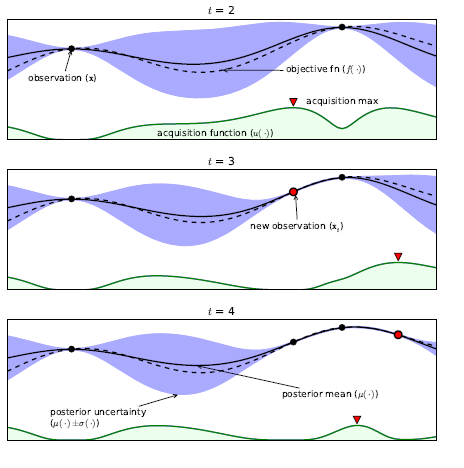
\includegraphics[width=.5\textwidth]{overview_1}
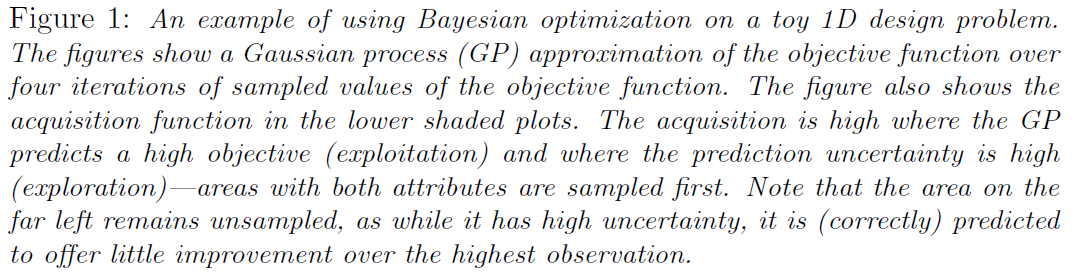
\includegraphics[width=.5\textwidth]{overview_2}
\end{center}
\end{frame}
%
\begin{frame}
\frametitle{References}
\begin{enumerate}
%\item[4.]
%Jonas Močkus, 1975, ``On the Bayes Methods for Seeking the Extremal Point''
\item[1.]
James Bergestra, et al., 2011, ``Algorithms for Hyper-Parameter Optimzation''
\item[2.]
Jasper Snoek, et al., 2012, ``Practical Bayesian Optimization of Machine Learning Algorithms''
\end{enumerate}
\end{frame}

%
\frame{Thank you}
\end{document}
